\chapter{绪论}
\section{研究背景和意义}
近年来深度学习技术快速发展,在图像识别、自然语言处理、自动驾驶、医疗诊断等领域取得了显著的进展和广泛的应用。现阶段的深度学习算法在准确性上已经可以达到很好的效果,但仍普遍存在过度自信问题(overconfident issue),即深度神经网络对其预测结果上往往过于自信,即使在它不熟悉的样本上,也可能错误地给出过高的预测概率。在一些高风险的领域,比如医疗诊断,自动驾驶等,一次错误的预测可能会带来严重的后果,过度自信问题使得神经网络在这些领域的应用仍然受到限制。因此,我们不仅希望模型能准确给出预测结果,还希望模型能给出一个值指示本次预测结果可靠程度,这就是神经网络的不确定性(Uncertainty)。一旦我们知道神经网络的本次预测不确定性很高,就可以在必要时引入人类监督或放弃高风险决策,规避风险和灾难性后果。

对神经网络不确定性的研究具有重大意义,不确定性研究有助于提升模型的鲁棒性,帮助模型更稳健、更可靠地应用于实际任务。通过对输入数据的不确定性建模,神经网络可以更加适应不同的输入分布,从而提高在多样化环境中的表现。这对应对分布外(out-of-distribution, OOD)数据尤其重要。在实际应用中,资源的合理分配往往需要依据决策的不确定性。例如,在医疗诊断中,当模型预测某些病例的不确定性较高时,可以优先将这些病例转交给医生进行人工检查,从而提高整体诊断的准确性和效率。神经网络作为“黑箱”模型,其缺乏可解释性的问题长期以来阻碍了其在关键领域的应用。通过不确定性研究,模型可以对自己的预测进行自我评价,为用户提供更直观的信心指标。这不仅有助于用户更好地理解和使用神经网络系统,还能增加对人工智能技术的信任。神经网络不确定性研究不仅是一个应用驱动的领域,也是一个重要的理论问题。通过研究不确定性,学术界和工业界能够更深入地理解神经网络的行为和特性。当前,不确定性研究已经催生了许多新的方法,例如深度高斯过程、贝叶斯神经网络、蒙特卡罗 dropout(MC dropout)、对抗训练等。这些方法不仅拓展了神经网络的理论基础,也为其他机器学习问题(如模型选择、主动学习)提供了新思路。


\section{不确定性的来源与分类}
神经网络不确定性(Uncertainty in Neural Networks)是指在神经网络的预测中,描述其对预测结果的置信程度或潜在错误的能力。量化神经网络的不确定性在许多实际应用中非常重要,尤其是在需要高可靠性和安全性的领域,如自动驾驶、医疗诊断和金融预测。神经网络中的不确定性通常可以分为两类\cite{abdar2021review}:\textbf{模型不确定性}(Model Uncertainty)和\textbf{ 数据不确定性}(Data Uncertainty)。

\textbf{模型不确定性},又称为\textbf{认知不确定性}(Epistemic Uncertainty),表示所训练的神经网络模型本身能力的局限性,可能来源于模型结构,训练过程,训练数据不足。当训练数据不足时,模型的参数未能很好地捕捉数据分布分布,导致预测的结果含有很大的模型不确定性。模型不确定性可以通过改变训练模型,优化训练过程,增加训练数据来减少。

\textbf{数据不确定性}(Data Uncertainty), 又称为\textbf{偶然不确定性}(Aleatoric Uncertainty),通常是由数据本身的随机性或噪声引起,可能来源于数据收集时噪声,数据标注时的错误。数据不确定性无法被消除。

值的注意的是,数据不确定性和模型不确定性并非绝对的,有时候二者可以相互转化\cite{hullermeier2021aleatoric}。本文重点研究模型的不确定性。

\begin{figure}[H]
    \centering
    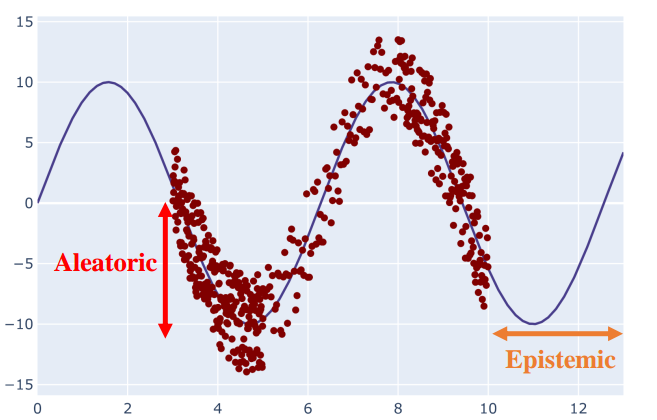
\includegraphics[width=0.75\linewidth]{assets/1-1.png}
    \caption{不确定性的来源与分类\cite{abdar2021review}
}
    \label{fig:enter-label}
\end{figure}

\section{不确定性研究的应用}
神经网络的不确定性研究(Uncertainty in Neural Networks)在许多应用场景中都具有重要价值,特别是在需要对预测结果的可靠性、稳定性和信心进行量化的任务中。传统的神经网络通常给出一个确定的预测结果(例如,分类标签或回归值),但并没有提供关于该结果的不确定性信息。而不确定性建模则能够量化模型对其预测的信心程度,这在多个领域中具有广泛的应用。

1. 自动驾驶

在自动驾驶系统中,车辆必须能够做出实时决策,基于感知模型(如卷积神经网络处理的摄像头图像、雷达、激光雷达等数据)预测和识别路况。然而,感知数据本身可能存在噪声,或者在复杂环境中不完全可靠。通过不确定性建模,自动驾驶系统可以识别哪些预测是可靠的,哪些可能需要进一步验证或修正。对不确定性的研究可以帮助确定对物体检测和追踪的信心程度,如识别行人、车辆和障碍物。判断模型在某些环境下的可靠性(例如,低光照或恶劣天气条件下的驾驶场景)。决策制定时结合不确定性,可以优先选择对结果不确定性较低的路径规划或行动。Hujie Pan等人\cite{pan2020towards}提出了一种改进的3D目标检测框架,结合不确定性估计方法,同时优化了算法性能与解释性。Di Feng等人\cite{feng2018towards}针对激光雷达(LiDAR)的3D车辆检测任务,提出了一种结合贝叶斯深度学习的方法,能够同时估计数据不确定性(Aleatoric uncertainty)和模型不确定性(Epistemic uncertainty),以提升检测性能和可靠性。通过不确定性信息优化预测结果,增强了自动驾驶系统在复杂环境中的安全性和稳健性。SalsaNext\cite{cortinhal2020salsanext} 是一种针对自动驾驶领域设计的高效、不确定性感知的语义分割模型,用于处理 LiDAR 点云数据。它在原有 SalsaNet 模型的基础上进行了改进,结合了注意力机制和贝叶斯学习框架,实现了更高的精度和不确定性估计能力,为自动驾驶中的环境感知提供了可靠的解决方案。

2. 医学影像分析

在医学影像分析中,如癌症检测或器官分割,模型不仅需要做出准确的预测,还需要能够提供关于其预测结果不确定性的估计。这对于医生和临床决策者至关重要,尤其是在面对复杂或模糊的医学影像时。在智能辅助诊断领域,对不确定的研究为医生提供关于某个影像分析结果(如肿瘤存在与否)的置信度,帮助医生判断是否需要进一步的检查或其他医学手段。在医学图像分割任务中,某些边界可能很模糊。通过不确定性估计,模型可以指出分割结果的可靠区域,辅助医生进行更准确的解读。Guotai Wang等人\cite{wang2019aleatoric}探讨如何结合测试时增强(Test-Time Augmentation, TTA)的方法,利用卷积神经网络(CNN)进行数据不确定性估计,从而提高医学图像分割的鲁棒性。在疾病预测方向上,基于患者历史数据和医学影像,模型预测某种疾病的风险,并通过不确定性量化本次预测的可信度,对不确定度高的预测引入专业医生的判断,可以减少误诊率,降低医疗事故的可能性。Maithra Raghu等人\cite{raghu2019direct}研究了不确定性对疾病糖尿病性视网膜病变(diabeticretinopathy,DR)诊断的改善。Tanya Nair等人\cite{nair2020exploring}探索了在多发性硬化症(MS)病变检测和分割中的应用上神经网络中不同的不确定性度量方法。文章提出了一种改进的U-Net架构,结合了四种不确定性度量:预测方差、蒙特卡罗(MC)样本方差、预测熵和互信息。这些不确定性度量有助于识别模型在预测中的不确定区域,并提高病变分割的准确性,尤其在医学影像分析中对于病变的检测至关重要。



3. 金融风控与预测

在金融行业中,模型预测的准确性对投资决策至关重要。不确定性量化有助于提高风险管理和预测系统的可靠性,尤其是在面对市场波动和不确定环境时。在信贷风险评估上,通过不确定性量化,金融机构能够识别贷款申请中哪些因素对违约预测有较高不确定性,从而采取更谨慎的风险管理措施。在市场预测上,量化市场趋势预测中的不确定性,帮助投资者做出更明智的决策,尤其在市场波动较大的情况下。在欺诈检测领域,在金融欺诈检测中,模型可以识别哪些交易行为具有更高的不确定性,从而引起额外的审查。\cite{wong2025quantifying}强调了不确定性量化对复杂金融时间序列预测的必要性,聚焦于时间序列中的波动性聚集特性(如资产回报率预测),提出了一种结合集成和 Evidential 的方法,显著提高了金融市场预测中的不确定性量化效果。这篇文章还重点分析了加密货币和股票的预测。

4. 自然语言处理(NLP)

在NLP任务中,神经网络通常需要处理复杂的文本和语言任务,不仅要生成准确的输出,还要提供预测的不确定性。例如,在机器翻译、情感分析或问答系统中,了解模型对结果的信心度对于理解其输出的可信度非常重要。在机器翻译领域,模型可以提供翻译的信心水平,帮助用户理解哪些翻译结果可靠,哪些可能需要进一步验证。在情感分析领域,评估情感分析模型的预测可信度,帮助商家了解用户评论中的潜在情感,尤其在情感极为复杂或模糊的情况下。在自动问答系统中,不确定性建模可以提供关于某个答案的置信度,帮助系统在遇到不确定的答案时请求进一步的信息或向用户确认。X. Han等人\cite{han2019attention} 提出一个基于注意力机制的神经网络框架,识别社交媒体文本中的不确定性,识别不确定性表达在情感分析、舆情监控和虚假信息检测等任务中非常重要。。

5. 机器人与自主系统

机器人在基于不完全的世界知识进行感知、决策、规划和行动时,可能会因错误导致任务失败或危及人类生命(如手术机器人、自动驾驶汽车等)。深度学习在机器人领域面临独特挑战,例如测试条件与训练分布不一致可能导致性能下降。因此,研究如何量化神经网络预测的不确定性,以避免灾难性错误,对于推动机器人技术的发展尤为重要。通过量化对环境状态或控制决策的信心,机器人可以决定是否需要进一步的信息,或者采取更保守的行动。在路径规划与控制方面,通过不确定性量化,机器人可以识别哪些路径或动作是更安全的,哪些决策可能会导致更高的风险。在环境感知方向上,在复杂环境中(例如多变的室内环境或户外环境),机器人可以基于不确定性评估来选择更可靠的传感器数据进行决策。\cite{peretroukhin2020smooth}提出了一种方法,用于在深度学习中实现对旋转群 SO(3) 的平滑表示,同时量化预测的不确定性。作者引入了一种概率分布表示,将旋转表示和不确定性建模相结合,以处理在三维旋转学习中的常见挑战。这种方法可以更准确地学习旋转,同时提供对模型置信度的估计,从而在计算机视觉任务(如姿态估计和物体跟踪)中表现出色。\cite{yang2020d3vo}通过联合学习场景深度、相机位姿以及不确定性估计,构建了一个端到端的框架。该模型利用深度神经网络提高视觉里程计在深度估计和位姿估计上的精度,同时引入不确定性评估以增强对环境变化的适应性。


\section{本文内容概要}
本文使用单一确定的网络建模不确定性,具体而言,是通过对训练集上神经网络提取的高维特征进行概率密度建模,当一个新的输入进入神经网络,所得到的新的高维特征在所建模的分布上的概率密度,可以作为模型不确定性的度量。这种方法DDU已经研究过了,本文是在DDU的基础上提升该方法的建模效果。

本文的研究工作从两个方面展开。首先,通过对梯度空间的分析,观察到OOD样本和训练集样本的差异,于是加入到输入图片中作为扰动,然后重新计算出对数概率密度,通过在OOD检测,对抗样本识别,主动学习等任务上的评估,可以看到该方法带来的提升。

另一方面,本文通过对特征空间的分析,使用辅助损失函数+交叉熵损失函数联合训练的方法,提升特征空间的类内紧密性和类间可分性,在联合训练后的特征空间上建模概率分布,并使用对数概率密度表征模型不确定性,通过在OOD检测任务上的评估,可以看到该方法的效果。

值的注意的是,因为数据不确定性和数据本身的噪声有关,所以本文控制数据集,主要研究神经网络的模型不确定性。
\section{章节安排}
本文共分五章内容组织。

第一部分主要是对不确定性的介绍,论述了不确定性的来源与分类,不确定性研究的意义和应用。

第二部分介绍了当前主流的建模不确定性的思路,主要包括贝叶斯神经网络,Ensemble方法,测试数据增强,单一确定性建模的方法。并介绍了这些方法是如何计算不确定性的,最后介绍一般是如何评估不确定性建模效果的。

第三部分主要介绍了基于输入扰动的一个改进,这个改进的来源于对梯度空间的分析,并在几个任务上评估了改进后的方法建模效果。

第四部分主要介绍了使用辅助损失函数联合训练的改进,想法来源于对特征空间的分析,最后在OOD检测任务上评估了改进后的方法的建模效果。

第五部分是总结和对未来的展望。
